% INTRODUÇÃO-------------------------------------------------------------------

\chapter{INTRODUÇÃO}
\label{chap:introducao}

% Importância de estudar o CNV
A variação no número de cópias (Copy Number Variation/CNVs) é um dos fatores que contribuem para a expansão e diversidade da família de genes, ela foi observada como alterações ocorridas em larga escada de inserções, deleções e duplicações na região genômica \cite{Perry2009,Zhao2013,Redon2006,Costain2016}. 
As CNVs podem ser identificada como uma variação neutra ou como modificadores de sucessibilidade a doenças \cite{Costain2016,Perry2009}.

% Estratégia de identificar CNV e ligação a doenças
A análise da região genômica pode ser realizada graças as tecnologias desenvolvidas para seu o sequenciamento, permitindo a observação de variantes de DNA \cite{Sathirapongsasuti2011}. Embora o sequenciamento completo do genoma seja uma abordagem utilizada para a investigação de CNVs, uma estratégia mais viável, econômica e eficiente no tempo para o estudo da base genética da doença é o sequenciamento completo do exoma, tendo em vista que 85\% dos variantes ligados a doenças mendelianas são encontrados nele \cite{Chong2015,Sathirapongsasuti2011,Fromer2012}.

% Ligação aos modelos estatísticos 
Devido a quantidade, complexidade e ruído dos dados obtidos a partir sequenciamento das regiões codificantes do genoma (exoma), muitas ferramentas de detecção de CNVs foram desenvolvidos para determinar os tipos, as quantidades e as localizações de variações \cite{Fromer2012,Tan2014}. Esses fatores podem ser alcançados com a utilização de modelos estatísticos na descoberta de variações no mapa de dados gerados no sequenciamento do exoma, essa é uma das abordagens que obteve mais sucesso na integração das ferramentas com o sequenciamento, devido a eficiência obtida \cite{Tan2014}. 

A utilização de modelos estatísticos aplicados para detecção de \textit{copy number variation} visa encontrar pontos de mudanças em uma representação gráfica dos dados, assim facilitando a determinação de uma variação de acordo com a localização do ponto de mudança \cite{Zhao2013}. Essa técnica se tornou popular, sendo desenvolvidos diversas ferramentas com o propósito de detectar pontos de mudanças (Change Point Detection/CPD) focadas na análise de CNV \cite{Olshen2004,Baldi2001,Girimurugan2018,Picard2011,Plagnol2012,Muggeo2010}. 

Apesar das diversas técnicas e ferramentas existentes de CPD, nenhuma delas é capaz de identificar todas as CNVs presentes no exoma \cite{Zhao2013}, entretanto a utilização de algumas dessas técnicas em determinada situação alcança uma maior efetividade ao encontrar variações. Essa diferença entre as técnicas pode ser vista ao comparar a execução de cinco algoritmos específicos de detecção de variações no número de cópias na \autoref{fig:ferramentas-cnv} \cite{Muggeo2010}. 

\begin{figure}[!htb] 
\centering 
\caption{Segmentação da linha celular de câncer de mama MDA157, onde cada linha representa um cromossomo, indexado ao lado esquerdo} 
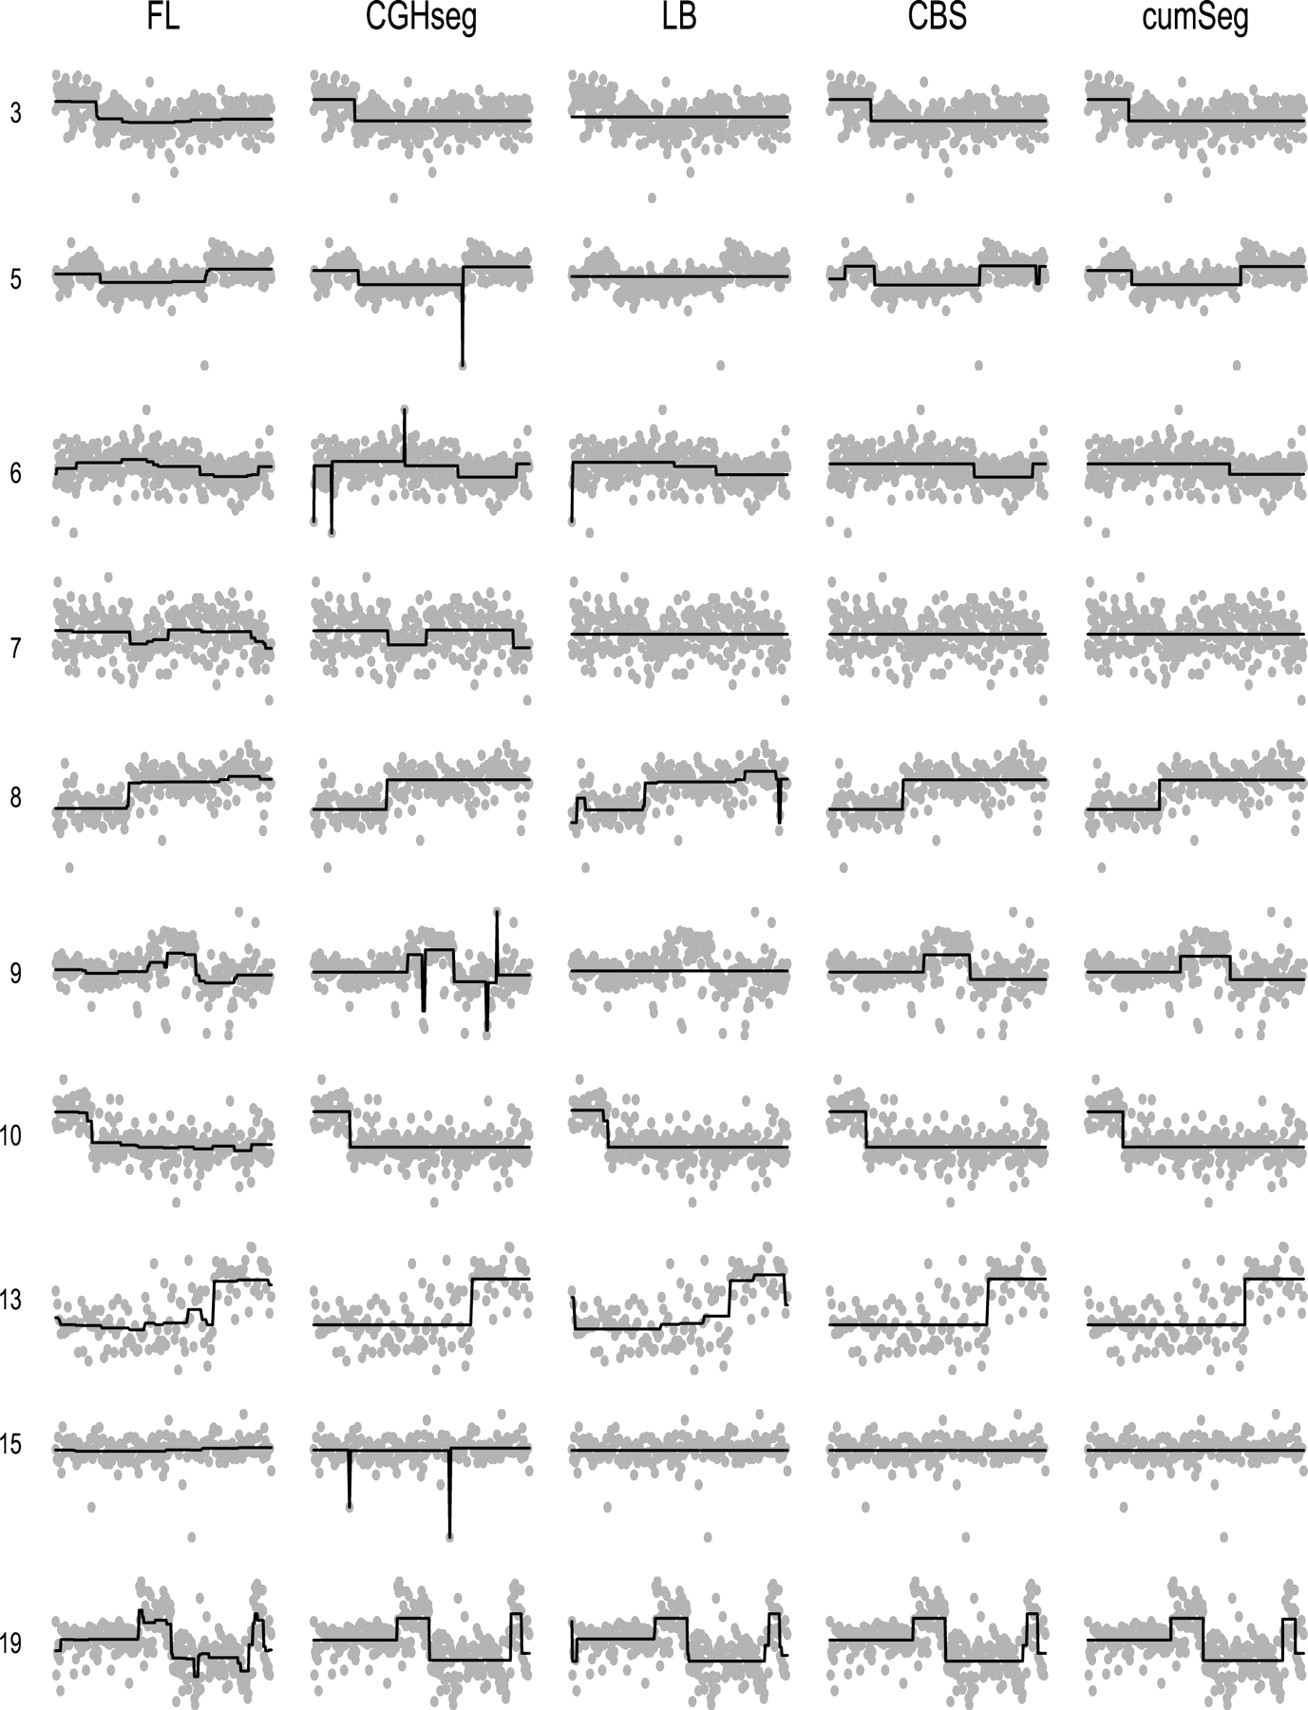
\includegraphics[width=0.8\textwidth]{./dados/figuras/ferramentas-cnv} 
\fonte{\cite{Muggeo2010}} 
\label{fig:ferramentas-cnv} 
\end{figure} 

A \autoref{fig:ferramentas-cnv} demostra que a variação da localização de pontos de mudanças relativos a um conjunto de dados (\textit{dataset}), pode apresentar mudanças de acordo com o algoritmo e a técnica implementada para análise na ferramenta. Esse mesmo efeito, também pode ser identificado em comparações de algoritmos de CPD \cite{Ducre-Robitaille2003,Reeves2007}. 

O desenvolvimento de técnicas de análises de CPD e CNVs, são frequentes na área da computação, sendo criados diversas teorias acerca dos assuntos em um período dois anos do ano atual \cite{Girimurugan2018,Uzai2019,Chu2019}, essa evolução pode ser observada sobre o viés da busca de melhoria contínua na eficiência em relação aos métodos existentes.



\section{JUSTIFICATIVA}



\section{OBJETIVOS}

\subsection{Objetivo Geral}

Aplicar o conceito de detecção de pontos de mudanças, utilizando diferentes abordagens técnicas desenvolvidas para segmentação de dados de uma série temporal, no contexto de anotação de variações no números de cópias nos dados do sequenciamento do exoma, para a obtenção de um ambiente integrado com diversos algoritmos de identificação de ponto de mudança em \textit{datasets} de um exoma.

\subsection{Objetivos Específicos}
	
\begin{itemize}
    \item Explicar a importância de \textit{copy number variation}.
    \item Descrever o conceito de \textit{change point detection}, caracterizando com exemplos, os algoritmos desenvolvidos para esse objetivo.
    \item Analisar a aplicabilidade dos algoritmos de CPD para a CNV, citando exemplos dos mesmos.
    \item Desenvolver um ambiente que dispõe de integrações com algoritmos de CPD
    \item Fornecer um algoritmo focado em leitura de dados de sequenciamento de DNA
\end{itemize}

\section{ORGANIZAÇÃO DO TEXTO}

Este trabalho se organiza da seguinte forma: 

\autoref{chap:introducao} - Introdução: Situa o leitor na área de pesquisa em que o trabalho é focado, definindo o porque do seu desenvolvimento e os objetivos a serem alcançados com a conclusão do projeto. 

\autoref{chap:fundamentacaoTeorica} - Revisão de Literatura: Apresenta uma pesquisa que contém conceitos e reflexões acerca dos principais conceitos referente ao trabalho proposto. Nele é apresentado temas relacionado ao trabalho proposto como a definição de exoma e a importância da utilização dele para descobertas de doenças (\autoref{sec:exoma}), o estudo acerca do surgimento e a evolução de tecnologias capazes de obter os componentes do genoma (\autoref{sec:sequenciamentoDoDna}), a definição de CNVs, ressaltando a importância do estudo e o uso dos métodos e ferramentas de detecção nessa variação genética (\autoref{sec:copyNumberVariation}), a formulação de uma das estratégias de detecção de CNV, a detecção de pontos de mudanças, sendo apresentado algoritmos específicos para utilização nesse tipo de situação (\autoref{sec:changePointDetection}) e a conceituação de matriz de confusão para aplicação em estudos com o objetivo de análise de performance \autoref{sec:matrizDeConfusao}. 

\autoref{chap:metodologia} - Metodologia: Discorre sobre os meios e procedimentos adotados, exemplificando e definindo a forma de desenvolvimento e as ferramentas envolvidas. 

\autoref{chap:planoDeTrabalho} - Plano de Trabalho: Expõe o cronograma adotado para o desenvolvimento do trabalho, disponibilizando o início e fim de um conjunto de atividades e sua descrição. 

\autoref{chap:conclusao} - Conclusão: Apresenta as considerações finais acerca do trabalho desenvolvido.